\chapter{Simulation Modules}

In the \bmad ``ecosystem'', various modules have been developed to
simulate machine hardware. This chapter provides documentation.

%-----------------------------------------------------------------
\section{Tune Tracker Simulator}
\index{tune tracker simulation}

\textit{\large [Tune tracker simulation developed by Michael Ehrlichman]}

The digital tune tracker (dTT) is device for determining the
fractional tune of a storage ring and exciting resonant beam
oscillations.  In short, the dTT starts with a beam position monitor
(BPM) to detect the beam oscillations. The signal from the BPM is feed
into a phase-locked loop (PLL) circuit which oscillates at the
oscillation frequency the beam. A signal from the PLL is used to
modulate a kicker to keep the beam oscillating at the beam's
oscillation frequency. The tune tracker is capable of exciting both
betatron and synchrotron oscillations.

In general, a PLL is a control system for matching the frequency of a
VCO to some incoming periodic reference signal.  It does this by
adjusting the frequency of the VCO according to the phase difference
between the VCO output and the reference signal.  A general diagram of
a PLL is shown in \fig{f:PLL}.

  \begin{figure}[bt]
  \centering
  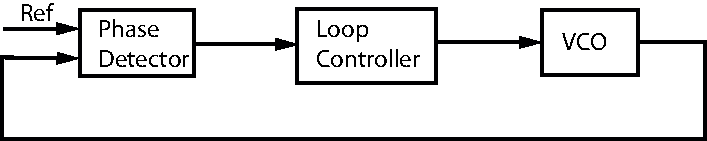
\includegraphics{PLL.pdf}
  \caption[General diagram of a phase lock loop.]{
General diagram of a phase lock loop. The loop adjusts the speed of a
VCO according to the phase difference between the VCO and an incoming
signal.}
  \label{f:PLL}
  \end{figure}

In \fig{f:PLL}, the phase detector compares the two incoming
signals, and outputs a signal that is proportional to the difference
in phase.  There are various ways to implement a phase detector.  The
tune tracker phase detector is a mixer followed by low-pass filter,
which will be discussed in more detail below.  The loop controller,
also known as a loop filter, is usually some combination of
(P)roportional, (I)ntegration, and (D)ifferentiation paths.  The loop
controller sums these paths, and the resulting signal is sent to the
VCO.  The output of the loop controller rises when the VCO is slower
than the reference, and drops when the VCO is faster.  The gains of
the three PID paths are adjusted to produce a control loop that is
stable and can efficiently lock onto the reference signal from some
incorrect initial frequency.  A real-world PLL also needs to track
perturbations to the reference frequency.

A diagram of the digital tune tracker is shown in
\fig{f:CdTT}.  This function takes in one new BPM measurement
per call, and returns a sinusoidal signal that has the same frequency
as the BPM signal.  The phase of the returned signal differs from the
phase of the BPM signal by $\phi_0$, the phase advance from position
at the BPM to position at the kicker on the next turn.

Comparing this diagram to the PLL in \fig{f:PLL}, the boxes
from {\it Subtract closed orbit offset} to the end of the {\it Low
Pass Filter} comprise the phase detector.  After the {\it Low Pass
Filter} to just before the {\it Gain Kvco} box comprises the loop
controller.  The {\it Gain Kvco} box comprises the VCO.  The feedback
loop consists of the update to $\omega$ that follows {\it Gain Kvco}.

\begin{sidewaysfigure}[tb]
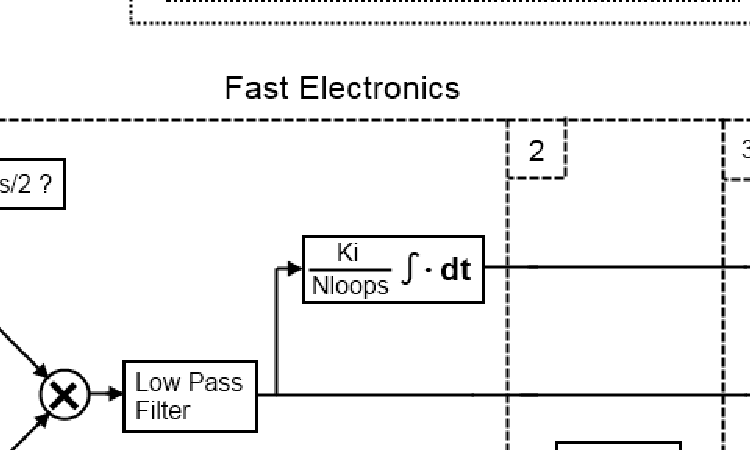
\includegraphics[width=\columnwidth]{TT-Flow.pdf}
\caption{
Flow chart of tune tracker module functions.}
\label{f:CdTT}
\end{sidewaysfigure}

\clearpage

\subsection{Tune Tracker Components.}
\begin{description}
\item[New BPM Meas.]  
This consists of one BPM measurement.  It is either horizontal or
vertical position at the BPM location.  It is assumed that each
measurement is separated by the same $\Delta t$, and that $\Delta t$
is an integer multiple of the ring period.

\item[Subtract closed orbit offset]  
Due to misalignments or the presence of wigglers, the closed orbit at
the BPM may be non-zero.  The closed orbit is subtracted from the
incoming data.  The closed orbit offset is a constant parameter set by
the user during initialization.

\item[Apply Gain G]  This block adjusts the incoming measurement such that,
\begin{equation*}
Meas.\ Out = \frac{Meas.\ In}{G}
\end{equation*}
The purpose of this block is to normalize the BPM measurements.  When
the tune tracker first starts, the amplitude of the beam oscillations
is small.  When the tune tracker is locked on, the amplitude of the
beam oscillations becomes large.  The set of loop controller gains
that allows the tune tracker to quickly lock onto the initially small
signal are not optimal when the beam oscillations are large.  This
normalization overcomes that problem, allowing for a set of loop
controller gains that are optimal both at start up and when
oscillations are large.

\item[Update Gain G]  This is a digital filter of the form,
\begin{equation*}
G = g_a \textrm{abs}\left(x\right) + \left(1-g_a\right)G\textrm{,}
\end{equation*}
which is a exponentially weighted moving average, or equivalently, a
low-pass filter.  $x$ is the incoming data point.  $g_a$ is a
hard coded time constant.  It is set so that $G$ equilibrates to the
rms beam size after about 10 periods.

\item[Fast Electronics]  
Fast electronics contains the components of the tune tracer that cycle
every few RF periods.  Whereas the rest of the tune tracker cycles
once per storage ring period, the fast electronics cycle every few RF
buckets.

\item[Prev Turn BPM Msmt]  Stores the previous turn's BPM measurement.

\item[Loop\# $\boldsymbol >$ $\boldsymbol N_{loops}/2$ ?]  
$N_{loops}$ is the number of times the fast electronics cycle every
storage ring period.  For the first half of these loops, the BPM
measurement from the previous turn is used.  For the last half, the
current BPM measurement is used.

\item[$\boldsymbol \sin\left(\psi\right)$]  
Sinusoid of the current modulator angle $\psi$.

\item[$\boldsymbol \psi$]  
Current modulator angle.  Updated at the end of every fast electronics loop.

\item[$\boldsymbol \times$ (times)]  
The BPM measurement and $\sin\left(\psi\right)$ are multiplied.  
Let the BPM signal be parameterized as $\cos\left(\omega_{beam}t\right)$, and 
write $\psi$ as $\omega_{vco}t$ so we have,
\begin{equation*}
\cos\left(\omega_{beam}t\right)\sin\left(\omega_{vco}t\right)\textrm{.}
\end{equation*}
A trig identity allows this to be written as,
\begin{equation*}
\frac{1}{2}\left(\sin\left(\left(\omega_{beam}+\omega_{vco}\right)t\right)-
\sin\left(\left(\omega_{beam}-\omega_{vco}\right)t\right)\right)\textrm{.}
\end{equation*}
If $\omega_{vco}$ is roughly $\omega_{beam}$, then the first $\sin$
term has roughly twice the beam frequency and the second term has a
very small frequency.  Therefore, passing the multiplied signal
through a low-pass filter removes the first term, leaving only the
second term.

In stable operation, $\omega_{vco}$ makes small amplitude oscillations
about $\omega_{beam}$.  In this case, the time integral of
$\left(\omega_{beam}-\omega_{vco}\right)t$ is small for all $t$, and a
small angle approximation for sine can be applied, and the output of
the low pass filter can be written as,
\begin{equation}
\left(\omega_{beam}-\omega_{vco}\right)t\textrm{,}
\end{equation}
which is proportional to the phase difference between the beam and the VCO.  Thus completes
the phase detector.

\item[$\boldsymbol{\frac{K_I}{N_{loops}}\int\cdot dt}$]  
This is the (I)ntegrated channel of the PID controller.  It integrates
the output of the phase detector, providing negative feedback.  If the
integrated phase is positive, the I channel slows the VCO down.  If
negative, it speeds the VCO up.  This channel is expected to
equilibrate to some non-zero value proportional to the difference
between the beam frequency and the VCO base frequency.

\item[Update $\boldsymbol{\psi}$] This increments the modulator phase according to,
\begin{equation}
\psi_{n+1}=\psi_n+\frac{T_{ring}}{N_{loops}}\omega_{vco}\textrm{.}
\end{equation}
In order to more accurately model things,
$\omega_{vco}$ is not updated within the fast electronics loop.

\item[Increment Loop\# by 1]  
Loop\# counts the number of times the fast electronics has been looped
through.

\item[If Loop\# $>$ $N_{loops}$, exit, else, loop]  
$N_{loops}$ is the number of times the fast electronics cycle per ring
period.

\item[Gain $\boldsymbol K_P$] 
This is the (P)roportional channel of the PID controller.  Is provides
negative feedback proportional to the output of the phase detector.
This channel responds faster than the integrated channel and so helps
the tune tracker track sudden changes in the frequency of the beam.
In practice, it also damps tune tracker oscillations.  If $K_P$ is too
small, the VCO may oscillate indefinitely around the fractional tune
of the beam.  See section~\sref{Tuning} below for more details.

\item[Gain $K_D$ $\times$ filtered derivative]  
This is the (D)ifferential channel of the PID controller.  Provides a
filtered first derivative of the output of the phase detector.  The
derivative is obtained a polynomial fitted to a history of the phase
detector output.  This channel can be used to smooth out the VCO
response and reduce overshoot.  See section~\sref{Tuning} below for
more details.

\item[$\boldsymbol +$ (sum)]  
This block sums the three output of the PID controller.

\item[Gain $K_{vco}$] 
This block represents the response of a voltage controlled oscillator.
The frequency of the output of a VCO is proportional to the voltage of
its input.  This block simply multiplies the output of the PID
controller by a constant.  This block updates the VCO frequency.

\item[$\boldsymbol{\sin\left(\psi+\psi_0\right)}$]  
Calculates kicker amplitude to be returned to the calling program.
This is the kick amplitude that should be used during the next turn.
$\psi_0$ is the phase advance from position at the BPM to position at
next turn's kicker.

\end{description}

\subsection{Tuning \label{Tuning}} Tuning the tune tracker consists of
adjusting the four gain parameters $K_P$, $K_I$, $K_D$, and $K_{vco}$.
The goal is to set the parameters such that the tune tracker quickly
locks onto the fractional tune of the beam, and settles quickly.  If
multiple tunes are being explored, then the size of the convergence
region is also important.  i.e.  The set of parameters should work for
a wide range of fractional tunes.  If jitter is being explored, then
the ability of the tune tracker to track a varying fractional tune is
also important.

A plot of the VCO speed during typical tune tracker operation is shown
in \fig{f:typ-tt}.  A tune tracker with a base period of 0.571
oscillations per ring period tracks a beam with a fractional tune of
0.5691.  Marked on this plot are 4 important features.  They are the
rise time, overshoot, settling rate, and precision.  The rise time is
how long it takes the tune tracker to approach the fractional tune of
the beam.  This is the location of the first peak after operation
begins.  The overshoot is the difference between the amplitude of the
first peak and the fractional tune.  The settling rate measures the
decay rate of the oscillations of the VCO about the fractional tune.
The precision is the noise in the VCO frequency.  The discrete nature
of the BPM measurements introduces noise at the phase detector stage.
The proportional channel adds this noise to the VCO frequency Shown in
Tab.~[\ref{t:pid-params}] is the effect increasing the PID controller
gains.

\begin{table}
\begin{tabular}{llllll} \toprule
Parameter&  Rise Time&        Overshoot&        Settling Rate&      Precision&  Stability Region\\ \midrule
$K_P$&      slight decrease&  decrease&         faster&             degrade&    shrink\\
$K_I$&      decrease&         increase&         slower&             no change&  shrink\\
$K_D$$^\textrm{see note}$&    slight increase&  slight decrease&  slightly faster&    degrade&    grow\\ \bottomrule
\end{tabular}
\caption[Effect on VCO response of increasing $K_P$, $K_I$, or $K_D$.]{
Effect on VCO response of increasing $K_P$, $K_I$, or $K_D$. 
{\it Note:} The effects of the derivative channel are theoritical and have not 
been verified extensively.}
\label{t:pid-params}
\end{table}

Stability region refers to the range of fractional tunes that the tune
tracker will converge to when starting from an initial tune in that
range.  In practice, if $K_P$ and $K_I$ are increased to optimize
response to a particular fractional tune, the stability region
will shrink.  e.g.  A large $K_P$ and $K_I$ could be found that very
quickly lock on to a fractional tune of 0.569, but are unstable for
0.622.  But note that a smaller $K_P$ and $K_I$ can be found that give
acceptible performance at 0.569, and also acceptible performance at
0.622 (and even 0.074).

\begin{figure}[tb]
\centering
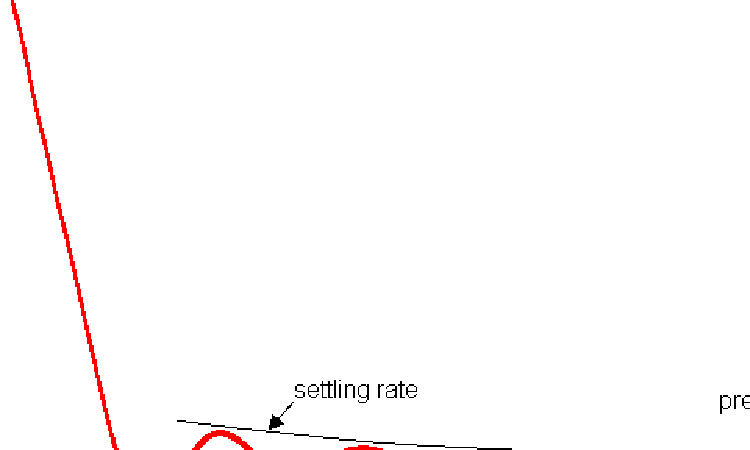
\includegraphics[scale=0.75]{vco-plot.pdf}
\caption[Plot of VCO response of typical tune tracker setup.]{
Plot of VCO response of typical tune tracker setup.  VCO base frequency is 0.571.
Beam fractional tune is 0.5691.}
\label{f:typ-tt}
\end{figure}

%----------------------------------------------------------------------

\subsection{Programmer Instructions}

This seciton contains instructions on how to implement the tune
tracker module and how to use the tune tracker driver program.  The
tune tracker is written as an object or class, and so supports
multiple instances.

After setting up the tune tracker in a program, it is best to first
verify that the tune tracker is efficiently locking onto the beam and
that the beam oscillations are indeed growing with time.  The tune
tracker should lock on after about 10,000 turns, and the beam
oscillations should reach equilibrium amplitude after about 10 damping
periods.

See the tune tracker section in the Physics chapter of this manual for
an example of how the VCO frequency should respond with time in a
successful implementation.  Guidelines for setting the gain parameters
are also located in the Physics chapter.

%-------------------------------------------------------------------------
\subsection{Tune Tracker Module}

The tune tracker module has four public functions.  They are,
\begin{alltt}
Function id = init_dTT(tt_param_struct)     !Constructor, creates new tune tracker 
                                            !instance, handles initialization.
                                            !Passed tt_param_struct, Returns id of 
                                            !created instance.
Function z = TT_update(bpm_msmt,id)         !Main function, passed one new BPM 
                                            !measurement and returns VCO modulator 
                                            !amplitude.
Subroutine dest_dTT(id)                     !Destructor, closes log files and 
                                            !deallocates memory.
                                            !Takes as argument id of instance 
                                            !to be destroyed.
Function z = get_dTT(name,id)               !Get function, name is either "wf", 
                                            !in which case the function returns 
                                            !the VCO frequency \(\omega0+\Delta\omega\), 
                                            !or "dw", in which case just \(\Delta\omega\)
                                            !is returned.
\end{alltt}

Pseudocode for a tune tracker implementation is below.
\begin{verbatim}
Populate tt_param_struct with tune tracker parameters.
id = init_dTT(tt_param_struct)
Loop over turns:
  Track once through the ring, obtain orbit.
  bpm_msmt = x or y at BPM location.
  z = TT_update(bpm_msmt,id)
  Adjust kicker amplitude (or cavity phase) according to z
dest_dTT(id)
\end{verbatim}

See {\tt tune\_tracker.f90} for the contents of {\tt tt\_param\_struct}.

If a horizontal or vertical tune tracker is to be implemented, the BPM
measrements should be the $x$ or $y$ coordinate at the BPM location,
and the kicks should be changes in $x'$ or $y'$ at the kicker
location.  If a longitudinal tune tracker is to be implemented the BPM
measurements should be the $x$ coordinate in a dispersive region, and
the kicks should be changes in phase at an RF cavity.  Similarly, if a
longitudinal tune tracker is being used in conjunction with a
horizontal tune tracker, the BPM of the horizontal tune tracker should
be placed in a region of low dispersion.  This will prevent the
horizontal tune tracker from inadvertantly locking onto the
synchrotron tune.

%-----------------------------------------------------------
\subsection{Tune Tracker Example Program}

An example program is located in {\tt
src/examples/tune\_tracker}. This program contains code for
implementing simultaneous horizontal, vertical, and longitudinal tune
trackers.

For most implementations of the tune tracker module, a good approach
would be to either use a modified version of the tune tracker example
program, or copy and paste code from the example program.  Keep in
mind that the example program implements multiple simultaneous tune
trackers.  An implementation of just one tune tracker would be much
simpler.

The example program performs the following steps.
\begin{enumerate}
\item 
Read in file which contains tune tracker parameters such as gains.
\item 
Parse lattice with {\tt twiss3} subroutines.  The {\tt twiss3} subroutines
are needed to obtain the longitudinal phase advance when implementing 
longitudinal tune trackers.
\item 
Check that the kick attribute of the kicker element is actually free.
\item 
Calculate phase advance from position at BPM to position at kicker.  Note that this 
is the phase of the kicker {\it on the next turn}.
\item 
Creates log files which record position at BPM and kicker, the VCO frequency,
and slope at the kicker.
\item
Loops over turns, passing BPM measurements to {\tt TT\_update} and
adjusting kicker amplitudes based on the returned value.  Note that it
will take the beam oscillations several damping times to equilibriate.
This often means tracking for several 10,000 turns.  Use of the save
state parameter may shorten simulation times in certain applications.
\item 
Calculates and FFT of the BPM data and records in log file. 
\end{enumerate}

Also located in {\tt src/examples/tune\_tracker} is an example .in
file that implements horizontal, vertical, and longitudinal tune
trackers.  The gains used in the .in file were selected for their
large convergence region.  More agressive tuning may lead to faster
lock on.  See the Physics section for details.

%----------------------------------------------------------------------------
\subsection{Save States}

If {\tt tt\_param\_struct\%useSaveState} is set to true, then the
destructor {\tt dest\_dTT} will save the tune tracker state variables
to a file called {\tt tt\_state.\#}.  Similarly, the constructor {\tt
init\_dTT} will set the state variables according to the save state
file.  The constructor will also return the beam coordinates to be
used at element zero of the ring.

Save states allow you to pick up where you left off, and not have to
wait for the beam oscillations to equilibriate.  For example, you
could have one program that tracks for 100,000 turns, allowing the
tune tracker to lock on and the beam excitation to equilibriate with
radiation damping.  The simulation writes a save state file which can
be used as a starting point for other simulations that perform studies
on the excited beam.

%-----------------------------------------------------------------
\section{Instrumental Measurements}
\label{s:meas.calc}
\index{measurement}

\bmad has the ability to simulate instrumental measurement errors
for orbit, dispersion, betatron phase, and coupling measurements.
The appropriate attributes are listed in \sref{s:meas.attrib} and
the conversion formulas are outlined below.

%-----------------------------------------------------------------
\subsection{Orbit Measurement}
\index{orbit!measurement}

For orbits, the relationship between measured position $(x, y)_{\text{meas}}$ and true position $(x,
y)_{true}$ is
\begin{equation}
  \begin{pmatrix}
    x \\ y
  \end{pmatrix}_{\! \text{meas}}
  =
  n_f \, 
  \begin{pmatrix}
    r_1 \\ r_2
  \end{pmatrix}
  +
  \bfM_m \, 
  \left[
  \begin{pmatrix}
    x \\ y
  \end{pmatrix}_{\! true}
  -
  \begin{pmatrix}
    x \\ y
  \end{pmatrix}_{\! 0}
  \right]
  \label{xynrr}
\end{equation}
where the Gaussian random numbers $r_1$ and $r_2$ are centered at zero and have unit width and the
factor $n_f$ represents the inherent noise in the measurement. In the above equation, $(x, y)_0$ 
represents a measurement offset and $\bfM_g$ is a ``gain'' matrix writen in the form
\begin{equation}
  \bfM_m
  =
  \begin{pmatrix}
     (1 + dg_x) \, \cos (\theta + \psi) & (1 + dg_x) \, \sin (\theta + \psi) \\
    -(1 + dg_y) \, \sin (\theta - \psi) & (1 + dg_y) \, \cos (\theta - \psi) 
  \end{pmatrix}
  \label{m1dg}
\end{equation}
Here $dg_x$ and $dg_y$ represent gain errors and the angles $\theta$ and $\psi$ are tilt and 
``crunch'' errors.

In the above equations, various quantities are writen as a difference between an ``error'' quantity
and a ``calibration'' quantity:
\begin{alignat}{1}
  x_0     &= x_{\text{off}} - x_{\text{calib}} \CRNO
  y_0     &= y_{\text{off}} - y_{\text{calib}} \CRNO
  \psi    &= \psi_{\text{err}}   - \psi_{\text{calib}} \CRNO
  \theta  &= \theta_{\text{err}} - \theta_{\text{calib}} \\
  dg_x    &= dg_{x,\text{err}} - dg_{x,\text{calib}} \CRNO
  dg_y    &= dg_{y,\text{err}} - dg_{y,\text{calib}} \nonumber
\end{alignat}
See \sref{s:meas.attrib} for the element attribute names that correspond to these quantities.

The calibration component is useful in a simulation where initally the error quantities are set to
represent the errors in the monitors. After this, analysis of orbit data with the machine in various
states can be used to calculate a best guess as to what the errors are. The calculated error values
can then be put in the calibration quantities. This represents a correction in software of the
errors in the monitors. Further simulations of orbit measurements will show how well the actual orbit
can be deduced from the measured orbit.

%-----------------------------------------------------------------
\subsection{Dispersion Measurement}
\label{Dispersion!measurement}

A dispersion measurement is considered to be the result of measuring the orbit at two different
energies. The measured values are then
\begin{equation}
  \begin{pmatrix}
    \eta_x \\ \eta_y
  \end{pmatrix}_{\! \text{meas}}
  =
  \frac{\sqrt{2} \, n_f}{dE/E} \, 
  \begin{pmatrix}
    r_1 \\ r_2
  \end{pmatrix}
  +
  \bfM_m \, \left[
  \begin{pmatrix}
    \eta_x \\ \eta_y
  \end{pmatrix}_{\! true}
  -
  \left(
  \begin{pmatrix}
    \eta_x \\ \eta_y
  \end{pmatrix}_{\! err}
  -
  \begin{pmatrix}
    \eta_x \\ \eta_y
  \end{pmatrix}_{\! calib}
  \right)
  \right]
\end{equation}
The factor of $\sqrt{2}$ comes from the fact that there are two measurements. $\bfM_m$ is given in \Eq{m1dg}.

%-----------------------------------------------------------------
\subsection{Coupling Measurement}
\label{Coupling!measurement}

The coupling measurement is considered to be the result of measuring
the beam at a detector over $N_s$ turns while the beam oscillates at a
normal mode frequency with some amplitude $A_{\text{osc}}$.  The
measured coupling is computed as follows. First, consider excitation
of the $a$-mode which can be written in the form:
\begin{equation}
  \begin{pmatrix}
    x_i \\
    y_i
  \end{pmatrix}_{\! \text{true}}
  =
  A_{\text{osc}} \,
  \begin{pmatrix}
    \cos \phi_i \\
    K_{22a} \, \cos \phi_i + K_{12a} \sin \phi_i
  \end{pmatrix}_{\! \text{true}}
  \label{xyapk}
\end{equation}
$i$ is the turn number and $\phi_i$ is the oscillation phase on the $i$\Th turn.
The coefficients $K_{22a}$ and $K_{12a}$ are related to the coupling $\bfCbar$ via
Sagan and Rubin\cite{b:coupling} Eq.~54:
\begin{alignat}{1}
  K_{22a} &= \frac{-\sqrt{\beta_b}}{\gamma \, \sqrt{\beta_a}} \, \bfCbar_{22} \CRNO
  K_{12a} &= \frac{-\sqrt{\beta_b}}{\gamma \, \sqrt{\beta_a}} \, \bfCbar_{12}
  \label{kabgbc}
\end{alignat}
To apply the measurement errors, consider the general case where the
beam's oscillations are split into two components: One component being
in-phase with some reference oscillator (which is oscillating with the
same frequency as the beam) and a component oscillating out-of-phase:
\begin{equation}
  \begin{pmatrix}
    x_i \\
    y_i
  \end{pmatrix}_{\! \text{true}}
  =
  \begin{pmatrix}
    q_{a1x} \\
    q_{a1y}
  \end{pmatrix}_{\! \text{true}}
  \, A_{\text{osc}} \, \cos (\phi_i + d\phi) +
  \begin{pmatrix}
    q_{a2x} \\
    q_{a2y}
  \end{pmatrix}_{\! \text{true}}
  \, A_{\text{osc}} \, \sin (\phi_i + d\phi)
  \label{xykkap}
\end{equation}
where $d\phi$ is the phase of the reference oscillator with respect to
the beam.  Comparing \Eq{xyapk} with \Eq{xykkap} gives the relation
\begin{alignat}{1}
  K_{22a} &= \frac{q_{a1x} \, q_{a1y} + q_{a2x} \, q_{a2y}}{q_{a1x}^2 + q_{a2x}^2} \CRNO
  K_{12a} &= \frac{q_{a1x} \, q_{a2y} - q_{a2x} \, q_{a1y}}{q_{a1x}^2 + q_{a2x}^2} 
  \label{kaqqqq}
\end{alignat}
This equation is general and can be applied in either the true or
measurement frame of reference.  \Eq{xynrr} can be used to transform
$(x_i, y_i)_{\text{true}}$ in \Eq{xyapk} to the measurement frame of
reference. Only the oscillating part is of interest.  Averaging over
many turns gives
\begin{equation}
  \begin{pmatrix}
    q_{a1x} \\
    q_{a1y}
  \end{pmatrix}_{\! \text{meas}}
  =  
  \bfM_m \, 
  \begin{pmatrix}
    q_{a1x} \\
    q_{a1y}
  \end{pmatrix}_{\! \text{true}}
  \comma \qquad
  \begin{pmatrix}
    q_{a2x} \\
    q_{a2y}
  \end{pmatrix}_{\! \text{meas}}
  =  
  \bfM_m \, 
  \begin{pmatrix}
    q_{a2x} \\
    q_{a2y}
  \end{pmatrix}_{\! \text{true}}
  \label{kkmkk}
\end{equation}
This neglects the measurement noise. A calculation shows that the noise gives a 
contribution to the measured $K_{22a}$ and $K_{12a}$ of
\begin{equation}
  K_{22a} \rightarrow K_{22a} + r_1 \, \frac{n_f}{N_s \, A_{\text{osc}}} 
  \comma \qquad
  K_{12a} \rightarrow K_{12a} + r_2 \, \frac{n_f}{N_s \, A_{\text{osc}}} 
  \label{kkrnn}
\end{equation}
Using the above equations, the transformation from the true
coupling to measured coupling is as follows: From a knowledge of the
true $\bfCbar$ and Twiss values, the true $K_{22a}$ and
$K_{12a}$ can be calculated via \Eq{kabgbc}. Since the value of $d\phi$
does not affect the final answer, $d\phi$ in \Eq{xykkap} is chosen to
be zero.  Comparing this to \Eq{xyapk} gives
\begin{equation}
  \begin{pmatrix}
    q_{a1x} \\
    q_{a1y}
  \end{pmatrix}_{\text{true}}
  =
  \begin{pmatrix}
    1 \\
    K_{22a}
  \end{pmatrix}_{\text{true}}
  \comma \qquad
  \begin{pmatrix}
    q_{a2x} \\
    q_{a2y}
  \end{pmatrix}_{\text{true}}
  =
  \begin{pmatrix}
    0 \\
    K_{12a}
  \end{pmatrix}_{\text{true}}
\end{equation}
Now \Eq{kkmkk} is used to convert to the measured $q$'s and
\Eq{kaqqqq} then gives the measured $K_{22a}$ and $K_{12a}$. Finally,
Applying \Eq{kkrnn} and then \Eq{kabgbc} gives the measured
$\bfCbar_{22}$ and $\bfCbar_{12}$. 

A similar procedure can be applied to $b$-mode oscillations to
calculate values for the measured $\bfCbar_{11}$ and $\bfCbar_{12}$.
$K_{11b}$ and $K_{12b}$ are defined by
\begin{equation}
  \begin{pmatrix}
    x_i \\
    y_i
  \end{pmatrix}_{\! \text{true}}
  =
  A_{\text{osc}} \,
  \begin{pmatrix}
    K_{11b} \, \cos \phi_i + K_{12b} \sin \phi_i \\
    \cos \phi_i
  \end{pmatrix}_{\! \text{true}}
  \label{xyakp}
\end{equation}
Comparing this to Sagan and Rubin\cite{b:coupling} Eq.~55 gives
\begin{alignat}{1}
  K_{11b} &= \frac{ \sqrt{\beta_a}}{\gamma \, \sqrt{\beta_b}} \, \bfCbar_{11} \CRNO
  K_{12b} &= \frac{-\sqrt{\beta_a}}{\gamma \, \sqrt{\beta_b}} \, \bfCbar_{12}
  \label{kbbgbc}
\end{alignat}
The $q_{x1b}$, $q_{y1b}$, $q_{x2b}$ and $q_{y2b}$ are defined by using
\Eq{xykkap} with the ``a'' subscript replaced by ``b''. The
relationship between $K$ and $q$ is then
\begin{alignat}{1}
  K_{11b} &= \frac{q_{b1y} \, q_{b1x} + q_{b2y} \, q_{b2x}}{q_{b1y}^2 + q_{b2y}^2} \CRNO
  K_{12b} &= \frac{q_{b1y} \, q_{b2x} - q_{b2y} \, q_{b1x}}{q_{b1y}^2 + q_{b2y}^2} 
  \label{kbqqqq}
\end{alignat}


%-----------------------------------------------------------------
\subsection{Phase Measurement}
\label{Phase!measurement}

Like the coupling measurement, the betatron phase measurement is
considered to be the result of measuring the beam at a detector over
$N_s$ turns while the beam oscillates at a normal mode frequency with
some amplitude $A_{\text{osc}}$.  Following the analysis of the
previous subsection, the phase $\phi$ is
\begin{equation}
  \begin{pmatrix}
    \phi_a \\
    \phi_b
  \end{pmatrix}_{\! \text{meas}}
  =
  \begin{pmatrix}
    \phi_a \\
    \phi_b
  \end{pmatrix}_{\! true}
  +
  \frac{n_f}{N_s \, A_{\text{osc}}} \, 
  \begin{pmatrix}
    r_1 \\ 
    r_2
  \end{pmatrix}
  -
  \begin{pmatrix}
    \tan^{-1} \left( \frac{q_{a2x}}{q_{a1x}} \right) \\
    \tan^{-1} \left( \frac{q_{b2y}}{q_{b1y}} \right)
  \end{pmatrix}_{\! \text{meas}}
\end{equation}
